\documentclass[11pt]{article}

\usepackage[english]{babel}                 %% hyphenation rules, spell-checker
\usepackage{amsmath,amssymb}                        %% macros like align* and pmatrix
\usepackage{graphicx,epstopdf}              %% for .eps graphs
\usepackage[official]{eurosym}              %% 1 \euro
\usepackage[a4paper,margin=2cm]{geometry}   %% margins
\usepackage{nameref}
\usepackage{hyperref}                       %% hyperlinks to urls
\usepackage{float}                    

\frenchspacing                              %% no extra space after period
\addtolength{\parskip}{0.5\baselineskip}    %% some white space between paragraphs
\setlength{\parindent}{0pt}                 %% but no indentation
\renewcommand{\baselinestretch}{1.1}        %% line spacing of TeX is small
\DeclareMathOperator{\E}{\mathbb{E}}
\DeclareMathOperator{\Var}{\text{Var}}
\DeclareMathOperator{\Cov}{\text{Cov}}


\title{Non-life --- Assignment NL5}  %% don't forget to change!

\author{
  Niels Keizer\footnote{Student number: 10910492}
  \quad and \quad
  Robert Jan Sopers\footnote{Student number: 0629049}
}

\date{\today}

\begin{document}

\maketitle

\subsection*{Q1}

We load the data, define $n,i,j$, execute the \verb|glm| command and find the coefficients, define \verb|alpha| and \verb|beta| and calculated the result of \verb|sum((Xij-fitted(Orig.CL))[i==5])| (observations minus fitted values for origination year 5). The output of \verb|R| is the following

\begin{verbatim}
> rm(list=ls(all=TRUE)); options(digits=6) ## housekeeping
> Xij <- scan(n=55) ## Data Taylor & Ashe (1983)
1: 357848 0766940 0610542 0482940 527326 574398 146342 139950 227229 067948
11: 352118 0884021 0933894 1183289 445745 320996 527804 266172 425046
20: 290507 1001799 0926219 1016654 750816 146923 495992 280405
28: 310608 1108250 0776189 1562400 272482 352053 206286
35: 443160 0693190 0991983 0769488 504851 470639
41: 396132 0937085 0847498 0805037 705960
46: 440832 0847631 1131398 1063269
50: 359480 1061648 1443370
53: 376686 0986608
55: 344014
Read 55 items
> 
> n <- length(Xij); TT <- trunc(sqrt(2*n))
> i <- rep(1:TT, TT:1); j <- sequence(TT:1)
> i <- as.factor(i); j <- as.factor(j)
> 
> Orig.CL <- glm(Xij~i+j, family=quasipoisson)
> coefs <- exp(coef(Orig.CL)); round(coefs,4)
(Intercept)	i2      i3      i4      i5      i6      i7      i8      i9      i10     j2 
270061.4156 1.3927  1.3787  1.3579  1.2452  1.3101  1.4509  1.7390  1.4462  1.2738  2.4906 
j3          j4          j5          j6          j7          j8          j9         j10 
2.6086      2.7899      1.5454      1.0833      0.9936      0.6740      1.0094      0.2516 
> alpha <- c(1, coefs[2:TT]) * coefs[1]
> beta <- c(1, coefs[(TT+1):(2*TT-1)])
> names(alpha) <- paste0("row",1:10); round(alpha)
row1   row2   row3   row4   row5   row6   row7   row8   row9  row10 
270061 376125 372325 366724 336287 353798 391842 469648 390561 344014 
> names(beta) <- paste0("col",1:10); round(beta, 4)
col1   col2   col3   col4   col5   col6   col7   col8   col9  col10 
1.0000 2.4906 2.6086 2.7899 1.5454 1.0833 0.9936 0.6740 1.0094 0.2516 
> 
> sum((Xij-fitted(Orig.CL))[i==5])
[1] -0.000169636
> 
\end{verbatim}
As expected by the marginal totals property the sum is (very close to) zero.

\subsection*{Q2}

We enter the code given in the question and obtain the following output. 

\begin{verbatim}
> Orig.fits <- outer(alpha, beta); round(Orig.fits)
col1    col2    col3    col4   col5   col6   col7   col8   col9  col10
row1  270061  672617  704494  753438 417350 292571 268344 182035 272606  67948
row2  376125  936779  981176 1049342 581260 407474 373732 253527 379669  94634
row3  372325  927316  971264 1038741 575388 403358 369957 250966 375833  93678
row4  366724  913365  956652 1023114 566731 397290 364391 247190 370179  92268
row5  336287  837559  877254  938200 519695 364316 334148 226674 339456  84611
row6  353798  881172  922933  987053 546756 383287 351548 238477 357132  89016
row7  391842  975923 1022175 1093189 605548 424501 389349 264121 395534  98588
row8  469648 1169707 1225143 1310258 725788 508792 466660 316566 474073 118164
row9  390561  972733 1018834 1089616 603569 423113 388076 263257 394241  98266
row10 344014  856804  897410  959756 531636 372687 341826 231882 347255  86555
> future <- row(Orig.fits) + col(Orig.fits) - 1 > TT
> (Orig.reserve <- sum(Orig.fits[future])) ## 18680856
[1] 18680856
> 
> row(Orig.fits)
       [,1] [,2] [,3] [,4] [,5]  [,6] [,7] [,8] [,9] [,10]
[1,]    1    1    1    1    1    1    1    1    1     1
[2,]    2    2    2    2    2    2    2    2    2     2
[3,]    3    3    3    3    3    3    3    3    3     3
[4,]    4    4    4    4    4    4    4    4    4     4
[5,]    5    5    5    5    5    5    5    5    5     5
[6,]    6    6    6    6    6    6    6    6    6     6
[7,]    7    7    7    7    7    7    7    7    7     7
[8,]    8    8    8    8    8    8    8    8    8     8
[9,]    9    9    9    9    9    9    9    9    9     9
[10,]   10   10   10   10   10   10   10   10   10    10
> matrix(as.numeric(future),10)
        [,1] [,2] [,3] [,4] [,5] [,6] [,7] [,8] [,9] [,10]
[1,]     0    0    0    0    0    0    0    0    0     0
[2,]     0    0    0    0    0    0    0    0    0     1
[3,]     0    0    0    0    0    0    0    0    1     1
[4,]     0    0    0    0    0    0    0    1    1     1
[5,]     0    0    0    0    0    0    1    1    1     1
[6,]     0    0    0    0    0    1    1    1    1     1
[7,]     0    0    0    0    1    1    1    1    1     1
[8,]     0    0    0    1    1    1    1    1    1     1
[9,]     0    0    1    1    1    1    1    1    1     1
[10,]    0    1    1    1    1    1    1    1    1     1
>
\end{verbatim}

The command \verb|row(Orig.fits)| gives the row number of each entry of the matrix \verb|Orig.fits| and therefore returns a matrix as seen above with the row number $i$ for each entry in row $i$. The future matrix given by \verb|matrix(as.numeric(future),10)| is the matrix with zeros for the past and known observations and ones for the future elements to be estimated. This matrix is produced by demanding that \verb|row(Orig.fits) + col(Orig.fits) - 1 > TT| and placing the results in a matrix with $10$ rows.


\subsection*{Q3}
We run the code and obtain the following output

\begin{verbatim}
> ij <- expand.grid(i=as.factor(1:TT),j=as.factor(1:TT))
> ij[c(1,5,10,19,35,67),]
i j
1   1 1
5   5 1
10 10 1
19  9 2
35  5 4
67  7 7
> mm <- matrix(predict(Orig.CL, ij, type="response"), TT); round(mm)
       [,1]    [,2]    [,3]    [,4]   [,5]   [,6]   [,7]   [,8]   [,9]  [,10]
[1,]  270061  672617  704494  753438 417350 292571 268344 182035 272606  67948
[2,]  376125  936779  981176 1049342 581260 407474 373732 253527 379669  94634
[3,]  372325  927316  971264 1038741 575388 403358 369957 250966 375833  93678
[4,]  366724  913365  956652 1023114 566731 397290 364391 247190 370179  92268
[5,]  336287  837559  877254  938200 519695 364316 334148 226674 339456  84611
[6,]  353798  881172  922933  987053 546756 383287 351548 238477 357132  89016
[7,]  391842  975923 1022175 1093189 605548 424501 389349 264121 395534  98588
[8,]  469648 1169707 1225143 1310258 725788 508792 466660 316566 474073 118164
[9,]  390561  972733 1018834 1089616 603569 423113 388076 263257 394241  98266
[10,] 344014  856804  897410  959756 531636 372687 341826 231882 347255  86555
> sum(Xij); sum(mm[row(mm)+col(mm)-1<=TT])
[1] 34358090
[1] 34358090
> sum(mm[row(mm)+col(mm)-1<=TT & row(mm)==TT-1])
[1] 1363294
\end{verbatim}

The first line of code assigns a data frame of all combinations of the factors \verb|i| and \verb|j| and the second line gives some examples stored in the object \verb|ij|. The third line creates via the function \verb|predict| the matrix of the fitted values by filling in the \verb|i|,\verb|j| values from the \verb|ij| object. The line \verb|sum(mm[row(mm)+col(mm)-1<=TT])| sums all fitted values over the past and therefore equals the sum of the observations. The last line sums the past entries of the \verb|mm| matrix via the restriction \verb|row(mm)+col(mm)-1<=TT| for the year of origin \verb|TT-1| = 9 via the restriction \verb|row(mm)==TT-1|.

\subsection*{Q4}

We run the code from the question and obtain the following output

\begin{verbatim}
> Prs.resid <- (Xij - fitted(Orig.CL)) / sqrt(fitted(Orig.CL))
> p <- 2*TT-1; phi.P <- sum(Prs.resid^2)/(n-p)
> Adj.Prs.resid <- Prs.resid * sqrt(n/(n-p))
> 
> birthday <- 820911; set.seed(birthday) ## do adjust this line
> nBoot <- 1000; payments <- reserves <- n.neg <- numeric(nBoot)
> for (boots in 1:nBoot){ ## running this will take 5--10 seconds
+   Ps.Xij <- sample(Adj.Prs.resid, n, replace=TRUE) ## 1
+   Ps.Xij <- Ps.Xij * sqrt(fitted(Orig.CL)) + fitted(Orig.CL) ## 2
+   number.neg <- sum(Ps.Xij<0)
+   Ps.Xij <- pmax(Ps.Xij, 0) ## Set obs < 0 to 0
+   Ps.CL <- glm(Ps.Xij~i+j, family=quasipoisson) ## 5
+   coefs <- exp(as.numeric(coef(Ps.CL)))
+   Ps.alpha <- c(1, coefs[2:TT]) * coefs[1]
+   Ps.beta <- c(1, coefs[(TT+1):(2*TT-1)])
+   Ps.fits <- outer(Ps.alpha, Ps.beta)
+   Ps.reserve <- sum(Ps.fits[future])
+   Ps.totpayments <- phi.P * rpois(1, Ps.reserve/phi.P) ## 11
+   reserves[boots] <- Ps.reserve ## 12
+   payments[boots] <- Ps.totpayments; n.neg[boots] <- number.neg}
> 
> sum(n.neg)
[1] 140
\end{verbatim}

From the $55 \times 1000 = 5500$ pseudo-observations generated there are $140$ negative pseudo-observations.

\subsection*{Q5}
To verify the statements in Remark 10.6.1 we let \verb|R| determine the minimum, maximum, mean and quantiles. The following output is obtained

\begin{verbatim}
> payments <- payments/1e6
> mean(payments)
[1] 18.9271
> min(payments)
[1] 8.10061
> max(payments)
[1] 32.455
> quantile(payments, c(0.25,0.75,0.05,0.95))
25%     75%      5%     95% 
16.8850 20.5671 14.5679 24.2492 
>
\end{verbatim}

These results are in line with the statements in Remark 10.6.1. The minimum is 8.1 mln, the maximum is 32.5 mln and the mean is 18.9 mln. The quantiles 25\% is at 16.9 mln, quantile 75\% at 20.6 mln, the 5\% quantile at 14.6 mln and the 95\% quantile at 24.2 mln. As the results in Remark 10.6.1 also show these results are very inaccurate.

\subsection*{Q6}
Changing the method construct a predictive distribution of the IBNR-reserve to be held to a gamma error distribution using the Hints given in the assignment we obtain the following output in \verb|R|

\begin{verbatim}
> Orig.CL.Gamma <- glm(Xij~i+j, family=Gamma(link=log))
> Prs.resid <- (Xij - fitted(Orig.CL.Gamma)) / fitted(Orig.CL.Gamma)
> p <- 2*TT-1; phi.P <- sum(Prs.resid^2)/(n-p)
> Adj.Prs.resid <- Prs.resid * sqrt(n/(n-p))
> 
> birthday <- 820911; set.seed(birthday) ## do adjust this line
> nBoot <- 1000; payments <- reserves <- n.neg <- numeric(nBoot)
> for (boots in 1:nBoot){ ## running this will take 5--10 seconds
+   Ps.Xij <- sample(Adj.Prs.resid, n, replace=TRUE) ## 1
+   Ps.Xij <- Ps.Xij * fitted(Orig.CL.Gamma) + fitted(Orig.CL.Gamma) ## 2
+   number.neg <- sum(Ps.Xij<0.01)
+   Ps.Xij <- pmax(Ps.Xij, 0.01) ## Set obs < 0.01 to 0.01
+   Ps.CL <- glm(Ps.Xij~i+j, family=Gamma(link=log)) ## 5
+   coefs <- exp(as.numeric(coef(Ps.CL)))
+   Ps.alpha <- c(1, coefs[2:TT]) * coefs[1]
+   Ps.beta <- c(1, coefs[(TT+1):(2*TT-1)])
+   Ps.fits <- outer(Ps.alpha, Ps.beta)
+   Ps.reserve <- sum(Ps.fits[future])
+   vec.Ps.fits <- Ps.fits[future]; h <- length(vec.Ps.fits)
+   Ps.totpayments <- sum(rgamma(h,1/phi.P,1/(vec.Ps.fits * phi.P)))
+   reserves[boots] <- Ps.reserve ## 12
+   payments[boots] <- Ps.totpayments; n.neg[boots] <- number.neg}
> 
> payments <- payments/1e6
> mean(payments)
[1] 18.3234
> quantile(payments, c(0.25,0.75,0.05,0.95))
25%     75%      5%     95% 
16.3441 19.9913 14.1696 23.2362 
> mean(payments)
[1] 18.3234
> sd(payments) 
[1] 2.79871
> 100 * sd(payments) / mean(payments) 
[1] 15.2739
> pp <- (payments-mean(payments))/sd(payments)
> sum(pp^3)/(nBoot-1)
[1] 0.545073
> sum(pp^4)/(nBoot-1) - 3
[1] 0.743627
\end{verbatim}

which gives a mean of 18.3 mln (18.7 mln for Poisson), a standard deviation of 2.8 mln/15.2\% coefficient of variation (sd 3 mln for Poisson, 15.8\% coefficient of variation) and a kurtois of 0.74 (1 for Poisson). These results of using the different error distributions can also be seen visually in Figure \ref{Figure_Question6}.

\begin{center}
	\begin{figure}[H]
		
		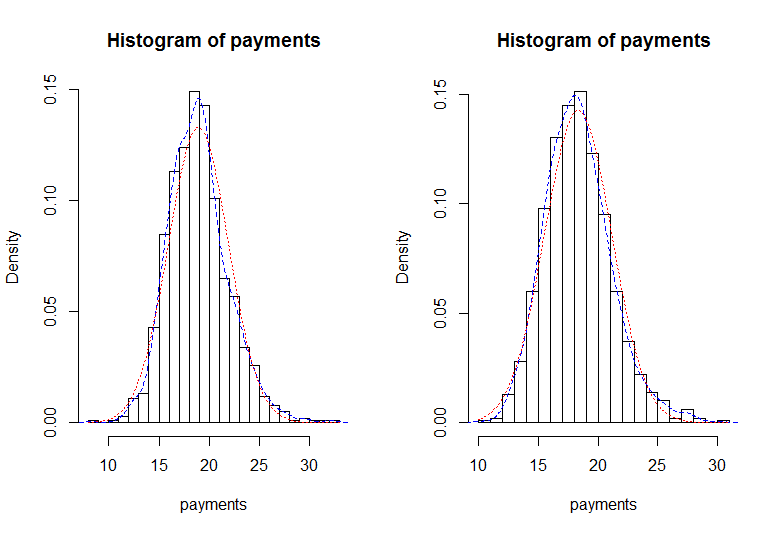
\includegraphics[scale=0.75]{Question6_NL5.png}
		
		\caption{Histograms of payments, left using Poisson error distribution and right gamma error distribution}
		\label{Figure_Question6}
		
	\end{figure}
\end{center}

The two distributions are very similar in all cumulants and this is clear from the Figure.


\subsection*{Q7}
We compute in \verb|R| the relative difference and obtain the following output 
\begin{verbatim}
> coefs <- exp(coef(Orig.CL.Gamma)); round(coefs,4)
(Intercept)  i2      i3      i4      i5      i6      i7      i8      i9      i10     j2 
284798.2615  1.3733  1.3277  1.1799  1.2593  1.3139  1.4224  1.5871  1.3595  1.2079  2.4808 
j3          j4          j5          j6          j7          j8          j9         j10 
2.5385      2.7116      1.5137      1.1172      0.9472      0.6378      0.9423      0.2386 
> alpha <- c(1, coefs[2:TT]) * coefs[1]
> beta <- c(1, coefs[(TT+1):(2*TT-1)])
> names(alpha) <- paste0("row",1:10); round(alpha)
row1   row2   row3   row4   row5   row6   row7   row8   row9  row10 
284798 391127 378115 336032 358657 374203 405084 452010 387195 344014 
> names(beta) <- paste0("col",1:10); round(beta, 4)
col1   col2   col3   col4   col5   col6   col7   col8   col9  col10 
1.0000 2.4808 2.5385 2.7116 1.5137 1.1172 0.9472 0.6378 0.9423 0.2386 
> (tapply(Xij/beta[j],i,sum)/tapply(Xij,i,length)-alpha)/alpha*1e6
1            2            3            4            5            6            7            
3.21291e+00 -1.84317e+00 -2.66958e+00 -1.26869e-02  8.81382e-01  3.90050e-01  5.67323e-02
8            9           10 
 -4.89973e-01 -4.76920e-02 -1.01521e-09 
>
\end{verbatim}

The largest deviation is about 3 in a million. This shows that the $\alpha_i$ parameters satisfy the DM-equations.

\subsection*{Q8}
We run the code from the question and comparing \verb|CL| and \verb|Orig.CL| via the summary we obtain the following output 

\begin{verbatim}
 > Xij.1 <- as.vector(t(xtabs(Xij~i+j))) ## stored row-wise as usual
 > ii <- rep(1:TT, each=TT); jj <- rep(1:TT, TT); future <- ii+jj-1 > TT
 > ii <- as.factor(ii); jj <- as.factor(jj)
 > Orig.CL <- glm(Xij~i+j, family=quasipoisson, epsilon = 1e-12)
 > CL <- glm(Xij.1~ii+jj, fam=quasipoisson, wei=as.numeric(!future))
 > 
 > summary(CL)
 
 Call:
 glm(formula = Xij.1 ~ ii + jj, family = quasipoisson, weights = as.numeric(!future))
 
 Deviance Residuals: 
 Min      1Q  Median      3Q     Max  
 -464.9   -31.5     0.0     0.0   494.3  
 
 Coefficients:
 Estimate Std. Error t value Pr(>|t|)    
 (Intercept) 12.50640    0.17292   72.32  < 2e-16 ***
 ii2          0.33127    0.15354    2.16   0.0377 *  
 ii3          0.32112    0.15772    2.04   0.0492 *  
 ii4          0.30596    0.16074    1.90   0.0650 .  
 ii5          0.21932    0.16797    1.31   0.1999    
 ii6          0.27008    0.17076    1.58   0.1225    
 ii7          0.37221    0.17445    2.13   0.0398 *  
 ii8          0.55333    0.18653    2.97   0.0053 ** 
 ii9          0.36893    0.23918    1.54   0.1317    
 ii10         0.24203    0.42756    0.57   0.5749    
 jj2          0.91253    0.14885    6.13  4.7e-07 ***
 jj3          0.95883    0.15257    6.28  2.9e-07 ***
 jj4          1.02600    0.15688    6.54  1.3e-07 ***
 jj5          0.43528    0.18391    2.37   0.0234 *  
 jj6          0.08006    0.21477    0.37   0.7115    
 jj7         -0.00638    0.23829   -0.03   0.9788    
 jj8         -0.39445    0.31029   -1.27   0.2118    
 jj9          0.00938    0.32025    0.03   0.9768    
 jj10        -1.37991    0.89669   -1.54   0.1326    
 ---
 Signif. codes:  0 ‘***’ 0.001 ‘**’ 0.01 ‘*’ 0.05 ‘.’ 0.1 ‘ ’ 1
 
 (Dispersion parameter for quasipoisson family taken to be 52601.9)
 
 Null deviance: 10699464  on 54  degrees of freedom
 Residual deviance:  1903014  on 36  degrees of freedom
 AIC: NA
 
 Number of Fisher Scoring iterations: 4
 
 Warning message:
 In summary.glm(CL) :
 observations with zero weight not used for calculating dispersion
 > summary(Orig.CL)
 
 Call:
 glm(formula = Xij ~ i + j, family = quasipoisson, epsilon = 1e-12)
 
 Deviance Residuals: 
 Min      1Q  Median      3Q     Max  
 -464.9  -123.7   -21.7   116.2   494.3  
 
 Coefficients:
 Estimate Std. Error t value Pr(>|t|)    
 (Intercept) 12.50640    0.17292   72.32  < 2e-16 ***
 i2           0.33127    0.15354    2.16   0.0377 *  
 i3           0.32112    0.15772    2.04   0.0492 *  
 i4           0.30596    0.16074    1.90   0.0650 .  
 i5           0.21932    0.16797    1.31   0.1999    
 i6           0.27008    0.17075    1.58   0.1225    
 i7           0.37221    0.17445    2.13   0.0398 *  
 i8           0.55333    0.18652    2.97   0.0053 ** 
 i9           0.36893    0.23918    1.54   0.1317    
 i10          0.24203    0.42756    0.57   0.5749    
 j2           0.91253    0.14885    6.13  4.7e-07 ***
 j3           0.95883    0.15257    6.28  2.9e-07 ***
 j4           1.02600    0.15688    6.54  1.3e-07 ***
 j5           0.43528    0.18391    2.37   0.0234 *  
 j6           0.08006    0.21477    0.37   0.7115    
 j7          -0.00638    0.23829   -0.03   0.9788    
 j8          -0.39445    0.31029   -1.27   0.2118    
 j9           0.00938    0.32025    0.03   0.9768    
 j10         -1.37991    0.89668   -1.54   0.1326    
 ---
 Signif. codes:  0 ‘***’ 0.001 ‘**’ 0.01 ‘*’ 0.05 ‘.’ 0.1 ‘ ’ 1
 
 (Dispersion parameter for quasipoisson family taken to be 52601.4)
 
 Null deviance: 10699464  on 54  degrees of freedom
 Residual deviance:  1903014  on 36  degrees of freedom
 AIC: NA
 
 Number of Fisher Scoring iterations: 5
 
 >
\end{verbatim}

The same results are obtained with \verb|CL| and \verb|Orig.CL| since the output is identical.

\subsection*{Q9}

We run the code and obtain the following output 

\begin{verbatim}
> p <- 2*TT-1
> phi.P <- sum((Xij - fitted(Orig.CL))^2 / fitted(Orig.CL))/(n-p) ## 1
> phi <- CL$deviance/CL$df.residual ## 2
> c(phi, phi.P) ## 52861.5 52601.4
[1] 52861.5 52601.4
> sum(resid(CL)^2)/(n-p) ## 3; "type=devi" is default
[1] 52861.5
> sum(resid(CL,type="pear")^2)/(n-p) ## 4
[1] 52601.4
> Prs.resid <- (Xij.1 - fitted(CL)) / sqrt(fitted(CL))
> sum(as.numeric(!future)*Prs.resid^2)/(n-p) ## 5
[1] 52601.4
> dev.resid2 <- 2 * (Xij.1*log(ifelse(Xij.1==0, 1, Xij.1/fitted(CL))) -
+                      (Xij.1 - fitted(CL))) ## cf. (9.29)
> sum(as.numeric(!future)*dev.resid2)/(n-p) ## 6
[1] 52861.5
> summary(CL)$dispersion ## 7 (the warning is reassuring)
[1] 52601.9
Warning message:
In summary.glm(CL) :
observations with zero weight not used for calculating dispersion
> summary(Orig.CL)$dispersion ## 8
[1] 52601.4

\end{verbatim}

From the output we see that method 1,4,5,7 and 8 are Pearson estimates and 2,3 and 6 are mean deviance estimates.

\subsection*{Q10}
Using a construction as proposed in the Hint we obtain the following output in \verb|R|

\begin{verbatim}
> mu.hat <- fitted(CL)*future
> Cov.beta <- vcov(CL)
Warning message:
In summary.glm(object, ...) :
observations with zero weight not used for calculating dispersion
> X <- model.matrix(CL)
> Cov.eta <- X %*% Cov.beta %*% t(X)
>   MSPE <- phi * sum(mu.hat) + t(mu.hat) %*% Cov.eta %*% mu.hat
>   cat("Total reserve =", round(sum(mu.hat)), "p.e. =", round(sqrt(MSPE)), "\n")
Total reserve = 18680856 p.e. = 2946484 
>   
>   
> for (r in 2:TT){
+   mu.r <- ifelse(ii==r,mu.hat,0) ## replace the elements of mu.hat not having rownr==r by 0
+   MSPE <- phi * sum(mu.r) + t(mu.r) %*% Cov.eta %*% mu.r;res <- round(sum(mu.r)); ## see above
+   cat("Year =", r, "\treserve =", round(res/1000),
+       "\tp.e./res. =", round(100*sqrt(MSPE)/res), "%\n") }
Year = 2 	reserve = 95 	p.e./res. = 116 %
Year = 3 	reserve = 470 	p.e./res. = 46 %
Year = 4 	reserve = 710 	p.e./res. = 37 %
Year = 5 	reserve = 985 	p.e./res. = 31 %
Year = 6 	reserve = 1419 	p.e./res. = 26 %
Year = 7 	reserve = 2178 	p.e./res. = 23 %
Year = 8 	reserve = 3920 	p.e./res. = 20 %
Year = 9 	reserve = 4279 	p.e./res. = 24 %
Year = 10 	reserve = 4626 	p.e./res. = 43 %
>
\end{verbatim}

which reproduces column 3 from Table 1 and 2 from England and Verrall (1999) exactly.

\subsection*{Q11}
We run the code and obtain the following output in \verb|R|

\begin{verbatim}
> rm(list=ls(all=TRUE)); Xij <- scan(n=36)
1: 156 37 6 5 3 2 1 0
9: 154 42 8 5 6 3 0
16: 178 63 14 5 3 1
22: 198 56 13 11 2
27: 206 49 9 5
31: 250 85 28
34: 252 44
36: 221
Read 36 items
> TT <- 8; i <- rep(1:TT, TT:1); j <- sequence(TT:1); k <- i+j-1
> fi <- as.factor(i); fj <- as.factor(j); fk <- as.factor(k)
> 
> ee <- c(28950,29754,26315,39442,38423,50268,44762,43541)
> Expo <- rep(ee, TT:1)
> 
> all(Expo == ee[i])
[1] TRUE
\end{verbatim}

The index \verb|i| in \verb|ee[i]| runs over the sequence created by \verb|i <- rep(1:TT, TT:1)| which consists of \verb|TT| times 1, \verb|TT-1| times 2, etc.. Since \verb|Expo| is created in the same manner (\verb|TT| repetitions of the first entry of \verb|ee|, \verb|TT-1| repetitions of the second entry of \verb|ee|) both vectors are equal for all entries.

\subsection*{Q12}
We fill in the dots and the output from \verb|R| is the following

\begin{verbatim}
> CL <- glm(Xij~fi+fj, quasipoisson) ## the Chain ladder model
> EE <- glm(Xij~fj+offset(log(Expo)),quasipoisson) ## the Exposure model
> scale <- CL$deviance / CL$df.residual ## mean-deviance estimate for phi
> Delta.Dev.Sc <- (EE$deviance - CL$deviance) / scale ## difference of scaled deviances for CL and EE
> Delta.df <- EE$df.residual - CL$df.residual ## difference of degrees of freedom for CL and EE
> reject <- Delta.Dev.Sc/scale > qchisq(0.95,Delta.df) ## TRUE if Delta.Dev.Sc > the chi^2 critical value
> cat("The exposure model", ifelse(reject, "is", "is not"), "rejected",
+     "since the scaled deviance gained by CL is\n",
+     round(Delta.Dev.Sc,1), "with", Delta.df, "extra parameters.\n")
The exposure model is not rejected since the scaled deviance gained by CL is
13.9 with 7 extra parameters.
>
\end{verbatim}

So the CL model is is not a significant improvement over the Exposure model. In the Exposure model the claims are modeled as proportional to $n_i \beta_j$ with $n_i$ the exposures in year $i$. The coefficients $\alpha_i$ of the \verb|CL| model are restricted in \verb|EE| via $\alpha_i = \frac{n_i}{n_1}$.

\subsection*{Q13}

Constructing the vectors \verb|alpha, beta, M| and \verb|delta| as prescribed with \verb|sum(beta)=sum(delta)=1| we obtain the following output in \verb|R|

\begin{verbatim}
> xtabs(round(100*(fitted(CL) - fitted(EE))/fitted(CL))~i+j)
  j
i       1   2   3   4   5   6   7   8
    1  -4  -5  -6  -6  -8 -12  -1   0
    2  -3  -4  -5  -5  -7 -11   0   0
    3  25  24  24  24  22  19   0   0
    4  -5  -6  -7  -7  -9   0   0   0
    5  -5  -6  -7  -7   0   0   0   0
    6   1   0  -1   0   0   0   0   0
    7  -3  -4   0   0   0   0   0   0
    8  -6   0   0   0   0   0   0   0
> round(coef(CL),2); round(coef(EE),2)
(Intercept)  fi2    fi3     fi4     fi5     fi6     fi7     fi8     fj2     fj3     fj4 
5.01	        0.04   0.23    0.30    0.27    0.60    0.45    0.39    -1.31   -2.70   -3.36 
fj5         fj6         fj7         fj8 
-3.90       -4.41       -5.72      -21.31 
(Intercept)  fj2         fj3         fj4         fj5         fj6         fj7         fj8 
-5.23       -1.30       -2.68       -3.34       -3.86       -4.33       -5.75      -21.35 
> 
> coefs.CL <- exp(coef(CL));
> alpha <- c(1, coefs.CL[2:TT]) * coefs.CL[1]
> beta <- c(1, coefs.CL[(TT+1):(2*TT-1)])
> alpha <- alpha*sum(beta); beta <- beta/sum(beta)
> 
> coefs.EE <- exp(coef(EE));
> M <- ee
> delta <- c(1,coefs.EE[2:TT])*coefs.EE[1]
> M <- M*sum(delta); delta <- delta/sum(delta)
> 
> round(100*(alpha%o%beta-M%o%delta)/(alpha%o%beta))
        fj2 fj3 fj4 fj5 fj6 fj7 fj8
    -4  -5  -6  -6  -8 -12  -1   0
fi2 -3  -4  -5  -5  -7 -11   0   1
fi3 25  24  24  24  22  19  27  28
fi4 -5  -6  -7  -7  -9 -13  -2  -1
fi5 -5  -6  -7  -7  -9 -13  -1  -1
fi6  1   0  -1  -1  -3  -7   4   5
fi7 -3  -4  -5  -5  -7 -11   1   1
fi8 -6  -6  -7  -8 -10 -14  -2  -2
> 
> round(100*(alpha-M)/alpha)
fi2 fi3 fi4 fi5 fi6 fi7 fi8 
-4  -3  25  -5  -5   0  -3  -6 
> round(100*(beta-delta)/beta)
fj2 fj3 fj4 fj5 fj6 fj7 fj8 
0   0  -1  -1  -4  -8   4   4 
\end{verbatim}
We see from the output of \verb|round(100*(alpha%o%beta-M%o%delta)/(alpha%o%beta))| that the differences are small between the models and the fitted values are similar for all rows and colums except for row 3 and colum 6. The differences are the result of the third entry of \verb|round(100*(alpha-M)/alpha)| and the 6th entry of \verb|round(100*(beta-delta)/beta)|.


\subsection*{Q14}
To compare the model with and without the term \verb|+fk| we do the anova call on the model with the \verb|+fk| term and without and obtain the following output in \verb|R|

\begin{verbatim}
> Three.off <- glm(Xij~offset(log(Expo))+fj+fi+fk, quasipoisson)
> anova(Three.off, test="Chisq")
Analysis of Deviance Table

Model: quasipoisson, link: log

Response: Xij

Terms added sequentially (first to last)


Df Deviance Resid. Df Resid. Dev Pr(>Chi)    
NULL                    35     3098.2             
fj    7   3041.5        28       56.7   <2e-16 ***
fi    7     22.6        21       34.2   0.0315 *  
fk    6     12.9        15       21.3   0.1856    
---
Signif. codes:  0 ‘***’ 0.001 ‘**’ 0.01 ‘*’ 0.05 ‘.’ 0.1 ‘ ’ 1
> 
> Three.off.without.fk <- glm(Xij~offset(log(Expo))+fj+fi, quasipoisson)
> anova(Three.off.without.fk, test="Chisq")
Analysis of Deviance Table

Model: quasipoisson, link: log

Response: Xij

Terms added sequentially (first to last)


Df Deviance Resid. Df Resid. Dev Pr(>Chi)    
NULL                    35     3098.2             
fj    7   3041.5        28       56.7   <2e-16 ***
fi    7     22.6        21       34.2   0.0532 .  
---
Signif. codes:  0 ‘***’ 0.001 ‘**’ 0.01 ‘*’ 0.05 ‘.’ 0.1 ‘ ’ 1
> 
> options(digits=7); summary(Three.off) #dispersion is 1.46782

Call:
glm(formula = Xij ~ offset(log(Expo)) + fj + fi + fk, family = quasipoisson)

Deviance Residuals: 
Min        1Q    Median        3Q       Max  
-1.56847  -0.51136  -0.01739   0.38596   2.43160  

Coefficients: (1 not defined because of singularities)
Estimate Std. Error t value Pr(>|t|)    
(Intercept)   -5.22347    0.09700 -53.850  < 2e-16 ***
fj2           -1.33452    0.07207 -18.518 9.60e-12 ***
fj3           -2.76272    0.14682 -18.817 7.62e-12 ***
fj4           -3.46343    0.23298 -14.866 2.20e-10 ***
fj5           -4.05421    0.34344 -11.805 5.41e-09 ***
fj6           -4.58245    0.51255  -8.941 2.13e-07 ***
fj7           -5.92674    1.21829  -4.865 0.000206 ***
fj8          -22.35244 4201.43685  -0.005 0.995825    
fi2            0.10724    0.16931   0.633 0.536004    
fi3            0.40860    0.17493   2.336 0.033800 *  
fi4           -0.08240    0.17121  -0.481 0.637259    
fi5           -0.12257    0.17055  -0.719 0.483385    
fi6           -0.00432    0.16387  -0.026 0.979318    
fi7           -0.21568    0.15830  -1.362 0.193160    
fi8           -0.05983    0.12669  -0.472 0.643568    
fk2           -0.13933    0.18226  -0.764 0.456456    
fk3           -0.17866    0.18643  -0.958 0.353091    
fk4            0.02194    0.17497   0.125 0.901896    
fk5            0.10201    0.16601   0.614 0.548098    
fk6           -0.04999    0.15420  -0.324 0.750267    
fk7            0.23054    0.13930   1.655 0.118689    
fk8                 NA         NA      NA       NA    
---
Signif. codes:  0 ‘***’ 0.001 ‘**’ 0.01 ‘*’ 0.05 ‘.’ 0.1 ‘ ’ 1

(Dispersion parameter for quasipoisson family taken to be 1.46782)

Null deviance: 3098.221  on 35  degrees of freedom
Residual deviance:   21.252  on 15  degrees of freedom
AIC: NA

Number of Fisher Scoring iterations: 15

>  summary(Three.off.without.fk) #dispersion is 1.62435 and deviance equal so lower scaled deviance

Call:
glm(formula = Xij ~ offset(log(Expo)) + fj + fi, family = quasipoisson)

Deviance Residuals: 
Min        1Q    Median        3Q       Max  
-2.51795  -0.73702  -0.08011   0.57321   2.11591  

Coefficients:
Estimate Std. Error t value Pr(>|t|)    
(Intercept) -5.268e+00  9.015e-02 -58.436  < 2e-16 ***
fj2         -1.310e+00  7.406e-02 -17.692 4.29e-14 ***
fj3         -2.700e+00  1.489e-01 -18.133 2.64e-14 ***
fj4         -3.357e+00  2.325e-01 -14.435 2.25e-12 ***
fj5         -3.902e+00  3.436e-01 -11.357 2.00e-10 ***
fj6         -4.407e+00  5.229e-01  -8.427 3.54e-08 ***
fj7         -5.717e+00  1.276e+00  -4.480 0.000206 ***
fj8         -2.131e+01  2.681e+03  -0.008 0.993733    
fi2          9.994e-03  1.232e-01   0.081 0.936130    
fi3          3.266e-01  1.179e-01   2.771 0.011459 *  
fi4         -1.052e-02  1.165e-01  -0.090 0.928895    
fi5         -9.808e-03  1.176e-01  -0.083 0.934318    
fi6          4.691e-02  1.109e-01   0.423 0.676604    
fi7          1.044e-02  1.156e-01   0.090 0.928908    
fi8         -1.530e-02  1.244e-01  -0.123 0.903299    
---
Signif. codes:  0 ‘***’ 0.001 ‘**’ 0.01 ‘*’ 0.05 ‘.’ 0.1 ‘ ’ 1

(Dispersion parameter for quasipoisson family taken to be 1.62435)

Null deviance: 3098.221  on 35  degrees of freedom
Residual deviance:   34.158  on 21  degrees of freedom
AIC: NA

Number of Fisher Scoring iterations: 14

>
\end{verbatim}

We see that in the model with the \verb|fk| term the exposure model is not rejected at 5\% level in favor of the \verb|CL| model but in the model without \verb|fk| the exposure model is rejected. The reason for this is the difference in the dispersion parameter. In the model with \verb|fk| the dispersion parameter is 1.46782 and in the model without 1.62435. This change in the dispersion parameter makes the unscaled deviance of 22.6 be significant in the model with \verb|fk| and not significant in the model without \verb|fk|.

\subsection*{Q15}
For year of development $j=8$ we have that the only observation is equal to 0. Therefore by the marginal totals property we have that $\beta_8 = 0$. But since we have a log link-function we should have that $\exp(\log \beta_8) = 0$. We expect the parameter $\beta_8$ therefore to be close to $\infty$. Calculating \verb|exp(coef(Three.off)[8])| in \verb|R| gives the output 
\begin{verbatim}
> exp(coef(Three.off)[8])
fj8 
1.960912e-10 
>
\end{verbatim}
which is close to zero.

\subsection*{Q16}
We also model the three-way model without offset and obtain the following output in \verb|R|
\begin{verbatim}
> Three.off.without.Offset <- glm(Xij~fj+fi+fk, quasipoisson)
> exp(Three.off.without.Offset$coefficients[1]) / exp(Three.off$coefficients[1])
(Intercept) 
28950 
>
\end{verbatim}
where \verb|exp(Three.off.without.Offset$coefficients[1]) / exp(Three.off$coefficients[1])| is equal to \verb|exp(+5.04986) / exp(-5.22347)| by inspecting of the coefficients of both models. The model without offset fits on $X_{11}$ and the model with offset on $\frac{X_{11}}{n_1}$ so the result of the division in \verb|R| is equal to $n_1 = 28950$. Therefore both models do lead to the same fitted value for the top-left observation as can be seen in the following \verb|R| output:

\begin{verbatim}
> exp(Three.off$coefficients[1])*(ee[1])
(Intercept) 
156 
> exp(Three.off.without.Offset$coefficients[1])
(Intercept) 
156 
>
\end{verbatim}

We calculate both fitted values for year of origin 2 and development year 1 in \verb|R| and obtain the following output 

\begin{verbatim}
> #Model zonder offset
> intersept.three.off.without.offset <- Three.off.without.Offset$coefficients[1]
> alpha2 <- Three.off.without.Offset$coefficients[9]
> beta1 <- 0
> gamma2 <- Three.off.without.Offset$coefficients[16]
> 
> exp(intersept.three.off.without.offset + alpha2 + beta1 + gamma2)
(Intercept) 
155.2694 
> 
> #Model met offset
> intersept.three.off <- Three.off$coefficients[1]
> alpha2 <- Three.off$coefficients[9]
> beta1 <- 0
> gamma2 <- Three.off$coefficients[16]
> 
> exp(intersept.three.off + alpha2 + beta1 + gamma2)*ee[2]
(Intercept) 
155.2694 

\end{verbatim}

We see that the fitted values coincide for both models.
	
\subsection*{Q17}
We create the dummy variable, construct the model and use \verb|anova| and obtain the following output 

\begin{verbatim}
> i.is.3 <- as.numeric(i==3)
> Three.off.Dummy3 <- glm(Xij~offset(log(Expo))+fj+i.is.3+fi, quasipoisson)
> anova(Three.off.Dummy3, test="Chisq")
Analysis of Deviance Table

Model: quasipoisson, link: log

Response: Xij

Terms added sequentially (first to last)


Df Deviance Resid. Df Resid. Dev  Pr(>Chi)    
NULL                      35    3098.22              
fj      7  3041.50        28      56.72 < 2.2e-16 ***
i.is.3  1    21.71        27      35.01 0.0002566 ***
fi      6     0.85        21      34.16 0.9975196    
---
Signif. codes:  0 ‘***’ 0.001 ‘**’ 0.01 ‘*’ 0.05 ‘.’ 0.1 ‘ ’ 1
> options(digits=7); summary(special3)

Call:
glm(formula = Xij ~ offset(log(Expo)) + fj + i.is.3 + fi, family = quasipoisson)

Deviance Residuals: 
Min        1Q    Median        3Q       Max  
-2.51795  -0.73702  -0.08011   0.57321   2.11591  

Coefficients: (1 not defined because of singularities)
Estimate Std. Error t value Pr(>|t|)    
(Intercept) -5.268e+00  9.015e-02 -58.436  < 2e-16 ***
fj2         -1.310e+00  7.406e-02 -17.692 4.29e-14 ***
fj3         -2.700e+00  1.489e-01 -18.133 2.64e-14 ***
fj4         -3.357e+00  2.325e-01 -14.435 2.25e-12 ***
fj5         -3.902e+00  3.436e-01 -11.357 2.00e-10 ***
fj6         -4.407e+00  5.229e-01  -8.427 3.54e-08 ***
fj7         -5.717e+00  1.276e+00  -4.480 0.000206 ***
fj8         -2.131e+01  2.681e+03  -0.008 0.993733    
i.is.3       3.266e-01  1.179e-01   2.771 0.011459 *  
fi2          9.994e-03  1.232e-01   0.081 0.936130    
fi3                 NA         NA      NA       NA    
fi4         -1.052e-02  1.165e-01  -0.090 0.928895    
fi5         -9.808e-03  1.176e-01  -0.083 0.934318    
fi6          4.691e-02  1.109e-01   0.423 0.676604    
fi7          1.044e-02  1.156e-01   0.090 0.928908    
fi8         -1.530e-02  1.244e-01  -0.123 0.903299    
---
Signif. codes:  0 ‘***’ 0.001 ‘**’ 0.01 ‘*’ 0.05 ‘.’ 0.1 ‘ ’ 1

(Dispersion parameter for quasipoisson family taken to be 1.62435)

Null deviance: 3098.221  on 35  degrees of freedom
Residual deviance:   34.158  on 21  degrees of freedom
AIC: NA

Number of Fisher Scoring iterations: 14

>
\end{verbatim}

The inclusion of the dummy variable is statistically significant at every level. The inclusion of the row factors after the dummy variable is not significant anymore. 

Adjusting the \verb|Expo| vector and repeating the previous steps gives the following output in \verb|R|

\begin{verbatim}
> Expo1 <- c(28950,29754,36315,39442,38423,50268,44762,43541)[i]
> Three.off.adjusted <- glm(Xij~offset(log(Expo1))+fj+i.is.3+fi, quasipoisson)
> anova(Three.off.adjusted, test="Chisq")
Analysis of Deviance Table

Model: quasipoisson, link: log

Response: Xij

Terms added sequentially (first to last)


Df Deviance Resid. Df Resid. Dev Pr(>Chi)    
NULL                      35    3129.79             
fj      7  3094.78        28      35.01   <2e-16 ***
i.is.3  1     0.00        27      35.01   0.9773    
fi      6     0.85        21      34.16   0.9975    
---
Signif. codes:  0 ‘***’ 0.001 ‘**’ 0.01 ‘*’ 0.05 ‘.’ 0.1 ‘ ’ 1

\end{verbatim}
The inclusion of the dummy variable is not statistically significant anymore after the adjustment of the \verb|Expo| vector. The inclusion of the row factors is still not significant.


\subsection*{Q18}

We repeat the code from the assignment, then we extract the \verb|alpha| and \verb|beta| values. Then we check if the sum over the past values obtained from \verb|alpha| and \verb|beta| equals the sum over the fitted values. Finally, we calculate the sum over the future estimated values.

\begin{verbatim}
> Xij <- scan(n=36)
1: 156 37  6  5 3 2 1 0
9: 154 42  8  5 6 3 0
16: 178 63 14  5 3 1
22: 198 56 13 11 2
27: 206 49  9  5
31: 250 85 28
34: 252 44
36: 221
Read 36 items
> TT <- 8; i <- rep(1:TT, TT:1); j <- sequence(TT:1); k <- i+j-1
> fi <- as.factor(i); fj <- as.factor(j); fk <- as.factor(k)
> ee <- c(28950,29754,31141,32443,34700,36268,37032,36637)
> Expo <- rep(ee, TT:1)
> CL <- glm(Xij~fi+fj, quasipoisson)
> EE <- glm(Xij~offset(log(Expo))+fj, quasipoisson)
> 
> cc <- exp(coef(CL))
> alpha <- cc[1] * c(1,cc[2:8]); names(alpha)[1] <- "fi1"
> beta <- c(1,cc[9:15]); names(beta)[1] <- "fj1"
> alpha <- alpha * sum(beta); beta <- beta / sum(beta)
> 
> i_tot <- rep(1:8, each=8)
> j_tot <- rep(1:8,8)
> k_tot <- i_tot+j_tot-1
> future <- k_tot>8
> 
> sum(CL$fitted.values)
[1] 2121
> sum(alpha[i_tot]*beta[j_tot]*!future)
[1] 2121
> sum(alpha[i_tot]*beta[j_tot]*future)
[1] 152.0312
\end{verbatim}

We see that the \verb|alpha| and \verb|beta| give the same past value as the model itself. We also see that we get the results that the assignment says we should get.

The total of the fitted values for past observations equals \verb|sum(Xij)| because of the marginal totals property.

\subsection*{Q19}

We run the code from the assignment and get the following result in \verb|R|.

\begin{verbatim}
> round(tapply(fitted.values(EE)-Xij,j,sum),6)
1 2 3 4 5 6 7 8 
0 0 0 0 0 0 0 0 
\end{verbatim}

The statement in \verb|R| is a sum over the difference between the observed and the fitted values for equal \verb|j|. These are the column sums. Because the \verb|EE| method uses dummy variables for the columns, the marginal totals property holds for the column sums.

\subsection*{Q20}

We execute the following code in \verb|R|, where we replace the dots by \verb|sum(fits) - sum(Xij)|.

\begin{verbatim}
> reserves <- numeric(); lasts <- c(171,181,191,201,211,271,261,251,241,231,221)
> for (last in lasts){
+   Xij[36] <- last
+   cc <- exp(coef(glm(Xij~fi+fj,quasipoisson)))
+   alpha <- c(1,cc[2:TT])*cc[1]; beta <- c(1,cc[(TT+1):(2*TT-1)])
+   fits <- (alpha %o% beta)
+   reserve <- sum(fits) - sum(Xij) ## the sum of the 'future' fitted values
+   reserves <- c(reserves, reserve) 
+ }
> rbind(lasts, reserves=round(reserves))
         [,1] [,2] [,3] [,4] [,5] [,6] [,7] [,8] [,9] [,10] [,11]
lasts     171  181  191  201  211  271  261  251  241   231   221
reserves  132  136  140  144  148  172  168  164  160   156   152
> plot(lasts, reserves); lines(range(lasts),range(reserves))
\end{verbatim}

This results in the following plot:

\begin{figure}[H]\label{fig:q20}
	\centering
	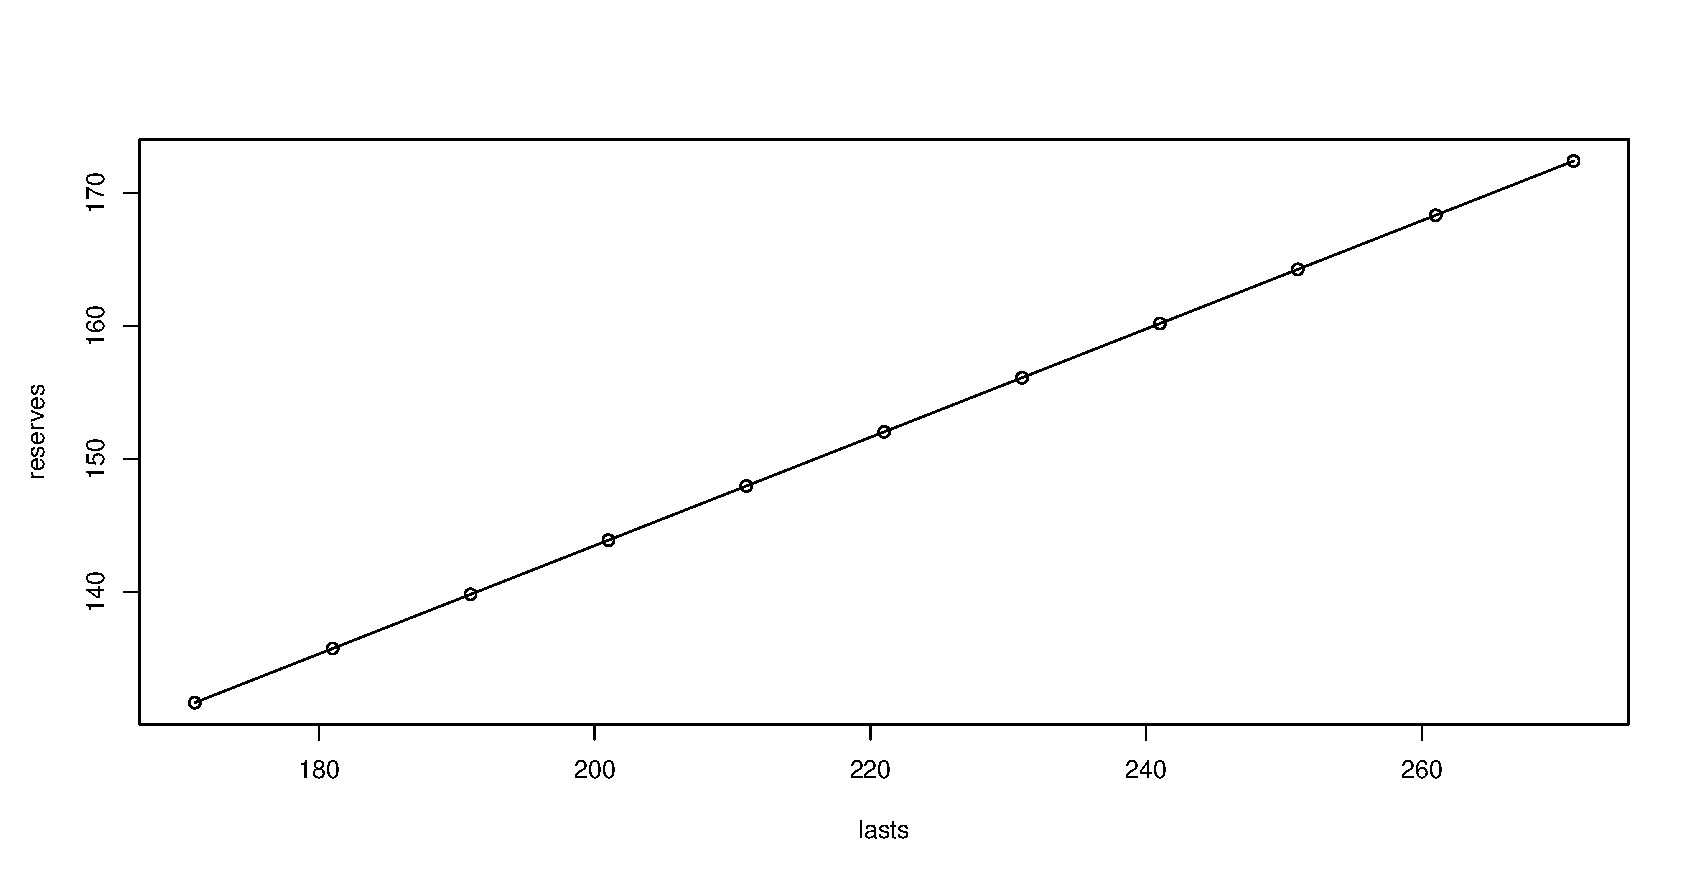
\includegraphics[width=0.8\textwidth]{fig_q20.eps}
	\caption{A plot of the chain ladder reserves against the last claim total.}
\end{figure}

\subsection*{Q21}

First we check the quality of a linear fit in \verb|R|.

\begin{verbatim}
> lin_fit <- lm(reserves~lasts)
> summary(lin_fit)

Call:
lm(formula = reserves ~ lasts)

Residuals:
Min         1Q     Median         3Q        Max 
-5.293e-12 -2.053e-12  7.766e-13  1.608e-12  5.461e-12 

Coefficients:
             Estimate Std. Error   t value Pr(>|t|)    
(Intercept) 6.198e+01  7.372e-12 8.409e+12   <2e-16 ***
lasts       4.074e-01  3.302e-14 1.234e+13   <2e-16 ***
---
Signif. codes:  0 ‘***’ 0.001 ‘**’ 0.01 ‘*’ 0.05 ‘.’ 0.1 ‘ ’ 1

Residual standard error: 3.463e-12 on 9 degrees of freedom
Multiple R-squared:      1,	Adjusted R-squared:      1 
F-statistic: 1.523e+26 on 1 and 9 DF,  p-value: < 2.2e-16
\end{verbatim}

From these results, we conclude that a linear fit is just about perfect.

We consider the final steps from Verbeek's algorithm for computing the CL coefficients. From the row sums, we see that $\alpha_{8}\beta_{1} = X_{8,1}$ ($X_{8,1} = R_{8}$). Because $\sum_{j} \beta_{j} = 1$ and the $\beta_{j}$ values have already been determined for $j \in (2, \ldots, 8)$, $\beta_{1}$ is independent from $X_{8,1}$. This implies $\alpha_{8} = X_{8,1}/\beta_{8}$, thus $\alpha_{8}$ is linearly dependent on $X_{8,1}$. By construction, all predicted values on row 8 are now also linearly dependent on $X_{8,1}$ and so is their sum. The total reserve is the sum of all predicted values, from which then follows that there is a linear relation between $X_{8,1}$ and the reserve.

We know that the sum over the predicted values of rows 1 to 7 are independent from $X_{8,1}$ and should therefore equal the intercept. We check this in \verb|R|.

\begin{verbatim}
> lin_fit$coefficients[1]
(Intercept) 
   61.98482 
> sum(alpha[1:7] %o% beta)-sum(Xij[i<=7])
[1] 61.98482
\end{verbatim}


\subsection*{Q22}

We construct the vector $\hat{M}$ with the following code:

\begin{verbatim}
M <- ee / ee[1] * alpha[1]
\end{verbatim}

\subsection*{Q23}

We copy the code from the assignment and fill the dots to obtain the following in \verb|R|.

\begin{verbatim}
> i_tot <- rep(1:8, each=8);j_tot <- rep(1:8,8)
> pred.CL <- alpha %*% t(beta); round(pred.CL, 4)
          fj1     fj2     fj3    fj4    fj5    fj6    fj7 fj8
[1,] 149.2060 40.2450 10.0252 5.2008 3.0131 1.8192 0.4907   0
[2,] 154.8901 41.7781 10.4071 5.3989 3.1279 1.8885 0.5093   0
[3,] 188.0126 50.7122 12.6327 6.5535 3.7968 2.2923 0.6183   0
[4,] 201.1539 54.2567 13.5156 7.0115 4.0622 2.4526 0.6615   0
[5,] 196.0964 52.8926 13.1758 6.8352 3.9600 2.3909 0.6448   0
[6,] 271.5200 73.2364 18.2436 9.4643 5.4832 3.3105 0.8929   0
[7,] 233.1209 62.8791 15.6635 8.1258 4.7077 2.8423 0.7666   0
[8,] 221.0000 59.6098 14.8491 7.7033 4.4630 2.6945 0.7267   0
> pred.BF <- M %*% t(beta); round(pred.BF, 4)
          fj1     fj2     fj3    fj4    fj5    fj6    fj7 fj8
[1,] 149.2060 40.2450 10.0252 5.2008 3.0131 1.8192 0.4907   0
[2,] 153.3498 41.3626 10.3036 5.3452 3.0968 1.8697 0.5043   0
[3,] 160.4983 43.2908 10.7840 5.5944 3.2412 1.9569 0.5278   0
[4,] 167.2087 45.1008 11.2348 5.8283 3.3767 2.0387 0.5499   0
[5,] 178.8411 48.2383 12.0164 6.2338 3.6116 2.1805 0.5881   0
[6,] 186.9225 50.4181 12.5594 6.5155 3.7748 2.2790 0.6147   0
[7,] 190.8600 51.4802 12.8240 6.6527 3.8543 2.3270 0.6276   0
[8,] 188.8242 50.9311 12.6872 6.5818 3.8132 2.3022 0.6209   0
> future <- xtabs(i_tot+j_tot-1>8~i_tot+j_tot)
> reserve.CL <- sum(pred.CL*future)
> reserve.BF <- sum(pred.BF*future)
> reserve.CL;reserve.BF
[1] 152.0312
[1] 125.9025
\end{verbatim}

We see that the reserve from the CL method is higher than the reserve from the BF method.

\subsection*{Q24}

We check that the retrofitted values from the BF method are not equal to the total observed sum.

\begin{verbatim}
> sum(pred.BF*(1-future))
[1] 1810.341
> sum(Xij)
[1] 2121
\end{verbatim}

This comes as no surprise, because the row coefficients where not determined using row dummies, in which case the marginal totals property would have held. The $\alpha$ parameters were replaced by exposure information and the $\beta$ parameters were kept, which means that the marginal totals property no longer holds and that the sums are not equal.

\subsection*{Q25}

We create a glm with coefficients proportional to the exposure for the rows.

\begin{verbatim}
CLoff <- glm(Xij~offset(log(Expo)+fj), quasipoisson)
\end{verbatim}

\subsection*{Q26}

We check that the retrofitted values now sum to the total observed values:

\begin{verbatim}
> sum(pred.off * (1-future)); sum(Xij)
[1] 2121
[1] 2121
\end{verbatim}

This is because the only parameters that were fitted are the column dummies. The row parameters were explained by an offset equal to the exposure. Because no parameters were replaced and the column dummies were constructed in such a manner that the marginal totals property holds over the columns, the marginal totals property also holds over the total sum. Which is \verb|sum(Xij)|.

\end{document}
